%!TEX root = ../book.tex

% ******************************* Part: Relational Databases ****************************

%this is a overarching PART that can be replicated to change overarching areas in the book
\part{Relational Databases}
\label{part:relationaldatabases}
This \lcnamecref{part:relationaldatabases} area allows me to write something about the PART.

% ******************************* Chapter: Introduction ****************************
\chapter{Introduction}
\label{chap:relational:introduction}
This book contains stuff about something.

\section{Background}
\begin{figure}[h]
    \centering
    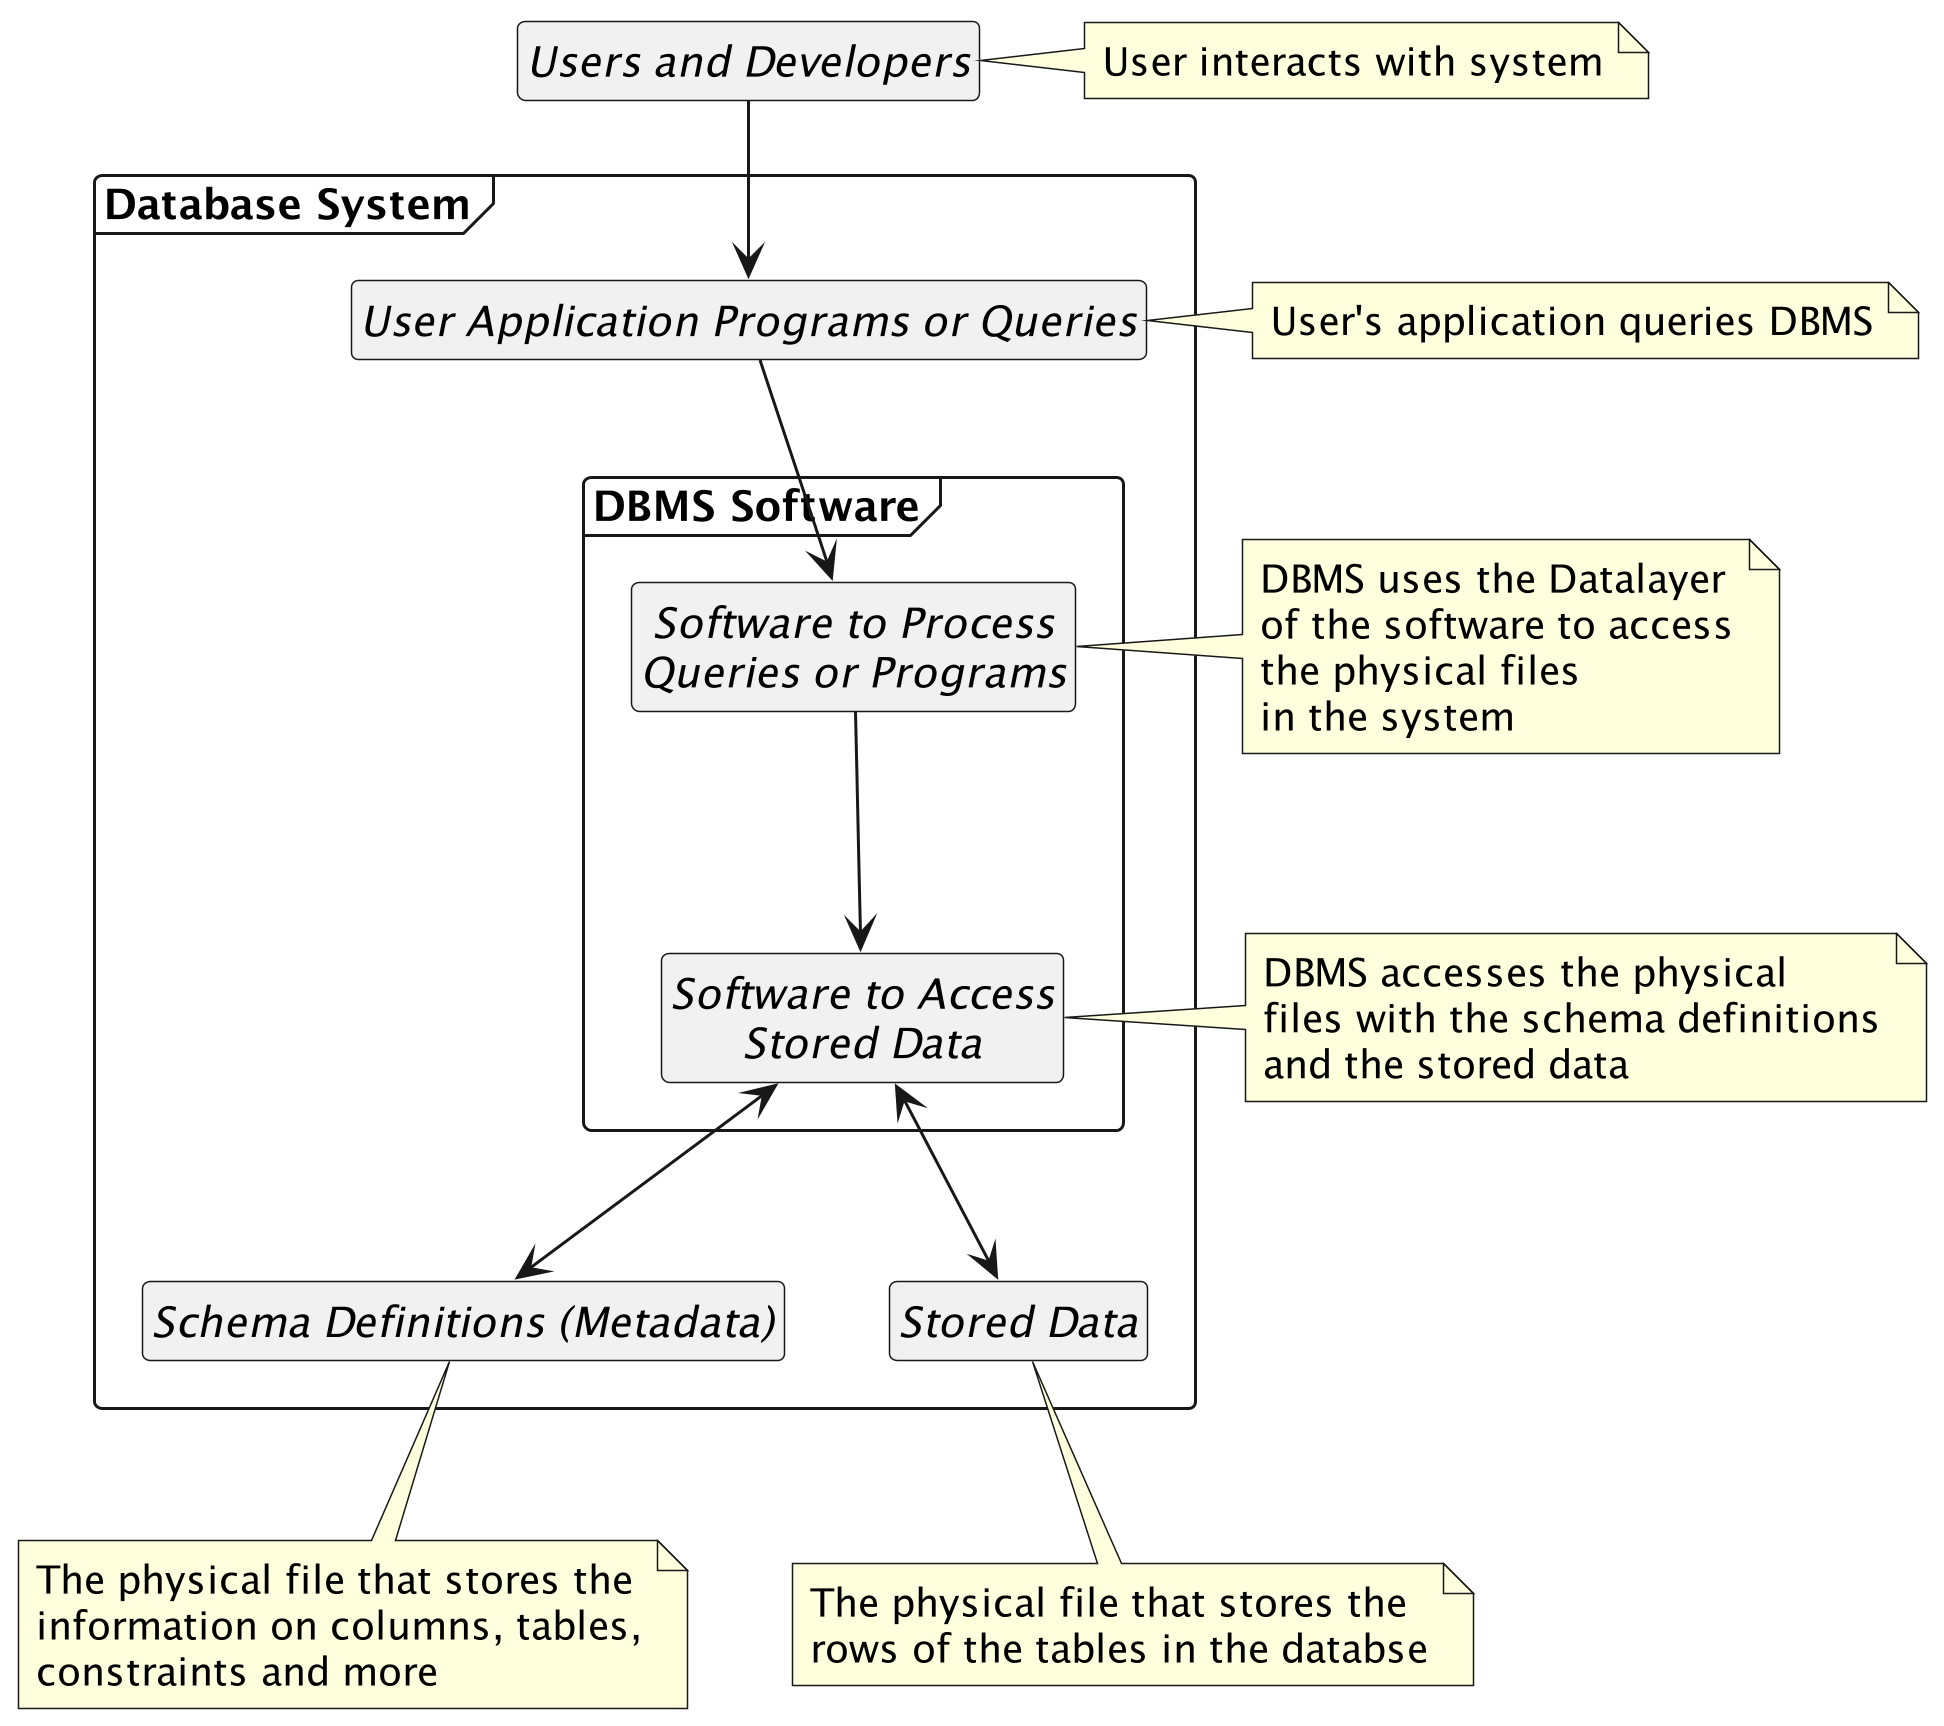
\includegraphics[width=1\textwidth]{content/1-relational-databases/figures/1.dbms-definitions.png}
    \caption{High Level Explanation of a Database Management System}
    \label{fig:1.dbms-definitions.png}
\end{figure}

\section{Getting Started}


% ******************************* Chapter: Relational Database Basics ****************************
\chapter{Relational Database Basics}
\label{chap:relational:relational-database-basics}
This chapter contains the basic building blocks to get started with basic relational databases.

\section{Creating your first database}
\section{CRUD Operations}
\subsection{Create Operations}
\subsection{Read Operations}
\subsection{Update Operations}
\subsection{Delete Operations}
\section{Joins and querying related tables}

% ******************************* Chapter: ER, EER Modeling and Database Design ****************************
\chapter{ER, EER Modeling and Database Design}
\label{chap:relational:eer-modeling-and-database-design}
This chapter teaches basic ER and ER modelling, and how to design a database from an ER model.

\section{The purpose of ER and EER modeling}
\section{Diagram Elements}
\section{ER versus EER modeling}
\section{Mapping to tables}

% ******************************* Chapter: Database Normalization ****************************
\chapter{Database Normalization}
\label{chap:relational:database-normalization}
This chapter teaches database normalization to the 4th normal form.

\section{What is database normalization?}
\section{Shorthand techniques}
\section{First normal form}
\section{Second normal form}
\section{Third normal form}
\section{Fourth normal form}
\section{Normalization of other formats}

% ******************************* Chapter: Advanced Relational Databases ****************************
\chapter{Advanced Relational Databases}
\label{chap:relational:advanced-relational-databases}
This chapter teaches advanced relational database concepts.

\section{Transactions}
\section{Indexes}
\section{Views}
\section{Stored Procedures}
\section{Triggers}
\section{User Defined Functions}
\section{Security}
\section{Performance Tuning}


